
\chapter{Космические корабли и станции: современные реалии 50-летней давности}
\label{ch:spacecraft-space-station}

Глава посвящена исследованию космических кораблей и станций на основе Викиданных. 
С помощью SPARQL-скриптов построен список отечественных кораблей и станций, 
нарисованы временные графики запуска кораблей в нашей стране и в мире за период с 1960 по 2021 год. 
Выполнена оценка полноты Викиданных, показавшая, 
что многие объекты имеют неправильное значение свойства 
\wdProperty{31}{частный случай понятия}.
\marginnote{<<Частный случай понятия>> или <<экземпляр>> 
    (англ. \emph{instance of})~--- это конкретный объект класса, категории, 
    это одно из основных свойств (отношений), используемых в Викиданных и позволяющих классифицировать объекты, 
    соотносить их разным <<классам>>, <<категориям>>.%
}


\section{Список космических кораблей и станций}

Построим запрос~\ref{lst:spaceships} для вывода списка всех космических кораблей и станций. 
Нам потребуются объекты \wdqName{космическая станция}{25956}, 
\wdqName{космический корабль}{40218} и отношение \wdProperty{31}{экземпляр}. 

\begin{lstlisting}[ language=SPARQL, numbers=none, caption={{\href{https://w.wiki/4d4f}{Список кораблей и станций}}\protect\footnotemark}, label=lst:spaceships, ]
# List of spacecraft (Q40218) and space station (Q25956)
SELECT  ?s ?sLabel ?typeLabel
WHERE
{
  VALUES ?type {wd:Q40218 wd:Q25956}
  ?s wdt:P31 ?type.  # Selecting the type of object
  SERVICE wikibase:label {bd:serviceParam wikibase:language"ru,en"}
}
\end{lstlisting}
\footnotetext{Найдено \num{145} объектов в 2021 году. SPARQL-запрос: \url{https://w.wiki/4d4f}}


\section{Глубина проработки объектов}

По состоянию на 2021 год на Викиданных 
наиболее полным и проработанным является космический корабль 
\wdqName{Аполлон-8}{184201}, 
имеющий 30 свойств\autocite{spacecraftProWD}. 
При этом всего всего по одному свойству имеют такие корабли, как: 
\wdqName{Europa Astrobiology Lander}{10491365}, 
\wdqName{Project Orbiter}{6514453}, 
\wdqName{LRK}{5961734}, 
\wdqName{EarthForce One}{5327028}\sidenote[][]{%
%
Отметим непростую судьбу объекта \wdqName{EarthForce One}{5327028}. 
Этот объект был создан в Викиданных ботом автоматически в 2013 году, 
поскольку существовала статья в Английской Википедии. 
Как написано на странице ``\href{https://en.wikipedia.org/wiki/EarthForce_One}{EarthForce One}'' 
в Английской Википедии, статья была удалена из-за отсутствия надёжных источников, 
доказывающих значимость объекта. 
А в Викиданных объект остался как неприкаянный. 
Подумайте над запросом, который вывел бы список аналогичных объектов Викиданных, 
не соответствующих ни одной статье Википедии.%
%
}, 
\wdqName{Союз ГВК}{60767924}, 
\wdqName{CubeSat for Solar Particles}{22907583}\autocite{spacecraftProWD}. 
Для поиска этой информации был использован запрос, построенный с помощью сервиса ProWD\autocite{spacecraftProWD}. 
Этот же сервис показал, что заполнение космических объектов неравномерное, 
большая часть заполнены менее, чем на 30\%\autocite{spacecraftProWD}. 


\section{Список отечественных кораблей и станций}
Найдём корабли и станции, сконструированные в СССР или России, 
с помощью запроса~\ref{lst:spaceshipsUSSR}.

\begin{lstlisting}[ language=SPARQL, 
                    numbers=none, 
                    caption={{\href{https://w.wiki/4d9c}{Список отечественных кораблей}}\protect\footnotemark}, 
                    label=lst:spaceshipsUSSR
                  ]
# List of Russian and USSR spacecrafts and stations
SELECT  ?spacecraft  ?spacecraftLabel 
WHERE
{
  {?spacecraft wdt:P31 wd:Q40218.} UNION #spacecraft
  {?spacecraft wdt:P31 wd:Q25956.} # and space station
  
  # Soviet Union and Russia
  VALUES ?ruCountries {wd:Q15180 wd:Q159}
  ?spacecraft wdt:P17 ?ruCountries. # related to Russian countries
  
  SERVICE wikibase:label {bd:serviceParam wikibase:language "ru,en"}
}
\end{lstlisting}
\footnotetext{Найдено три отечественных корабля и станции 
в 2017 году и \num{25}~--- в 2021 году. SPARQL-запрос: \href{https://w.wiki/4BbY}{https://w.wiki/4d9c}}


\section{Анализ полноты Викиданных}

Проанализируем степень заполнения Викиданных в области отечественных космических кораблей и станций. 
Если по запросу~\ref{lst:spaceships} обо всех кораблях и станциях было получено 145 результатов, 
то по запросу~\ref{lst:spaceshipsUSSR} об отечественных объектах~--- всего 25. 

В статьях Русской Википедии <<\href{https://ru.wikipedia.org/?curid=1218094}{Космическая программа СССР}>> и <<\href{https://ru.wikipedia.org/?curid=6147222}{Космонавтика России}>> можно насчитать как минимум 45 космических кораблей, спроектированных в СССР и России. То есть в Викиданных представлено менее половины от всех отечественных кораблей, однако ситуация в 2021 стала значительно лучше по сравнению с 2017 годом, когда по запросу~\ref{lst:spaceshipsUSSR} выдавалось менее 10\% от всех кораблей. 


\section{Временные графики освоения космоса в~нашей стране и мире}

Временной (с 1960-х годов) 
график запуска космических аппаратов в нашей стране (рис.~\ref{fig:launchesRussia5years}) 
построен с помощью запроса~\ref{lst:launchesRussia5years}.%

Ранее в запросах для получения каких-либо списков мы использовали свойство \wdProperty{31}{экземпляр}. 
В запросе~\ref{lst:launchesRussia5years} мы обошлись без этого свойства за счёт использования отношения 
\wdProperty{619}{<<дата запуска космического корабля>>} в строке 8 
для обхода и подсчёта таких объектов, которые были запущены в космос.  

Логический оператор \lstinline|UNION| в строках 5--6 
позволяет объединить советские и российские запуски космолётов. 

Если бы в запросе вместо переменной \lstinline|?lapse| оставалась~--- \lstinline|?year| (строки 3 и 10), 
то мы получили бы на рис.~\ref{fig:launchesRussia5years} 
число запусков за каждый год. 
Благодаря функции округления \lstinline|FLOOR()| 
и группировке%
\sidenote[][]{
%
В строке 13 запроса~\ref{lst:launchesRussia5years} 
запущенные в космос объекты группируются командой: 
\mbox{\lstinline|GROUP BY ?lapse|.}\newline
То, что группировка идёт именно по пятилеткам, а не, например, шестилеткам, 
определяется в строке 10, где переменная \lstinline|?year| делится на 5, округляется и умножается на 5.%
%
}, 
объекты \lstinline|?item|, имеющие запуски, группируются за пятилетний период, 
и в переменную \lstinline|?quantity| записывается число этих объектов, 
подсчитанное с помощью функции \lstinline|COUNT()|.

\marginnote[3cm]{
%%%%%%%%%%%%%%%% Упражнение 1 %%%%%%%%%%%%%%%% 
Сколько кораблей было запущено в~СССР в~1960-е, 1970-е и 1980-е годы?

См. ответ~\ref{answer:launches_USSR} на с.~\pageref{answer:launches_USSR}.
}
\begin{lstlisting}[ language=SPARQL, 
                    caption={{\href{https://w.wiki/4QGX}{Запуски космических кораблей в СССР и России}}\protect\footnotemark}, 
                    label=lst:launchesRussia5years,
                    texcl
                  ]
# The number of spacecraft launches in Russia every 5 years
#defaultView:BarChart
SELECT (STR(?lapse) AS ?lapse_str) (COUNT(?item) AS ?quantity)
WHERE {                  # spacecraft belongs to
        {?item wdt:P17 wd:Q15180} # Soviet Union
  UNION {?item wdt:P17 wd:Q159}.  # or Russia
  
  ?item wdt:P619 ?launch. # date of spacecraft launch
  BIND( YEAR(?launch) AS ?year) 
  BIND(FLOOR(?year/5)*5 AS ?lapse) # count for each 5 years
SERVICE wikibase:label {bd:serviceParam wikibase:language "ru,en"}
} 
GROUP BY ?lapse
ORDER BY ?lapse # Order 1970, 1975, 1980, ...
\end{lstlisting}
\footnotetext{Найдено \num{14} пятилеток. SPARQL-запрос: \href{https://w.wiki/4QGX}{https://w.wiki/4QGX}}

\begin{figure*}[h!]
  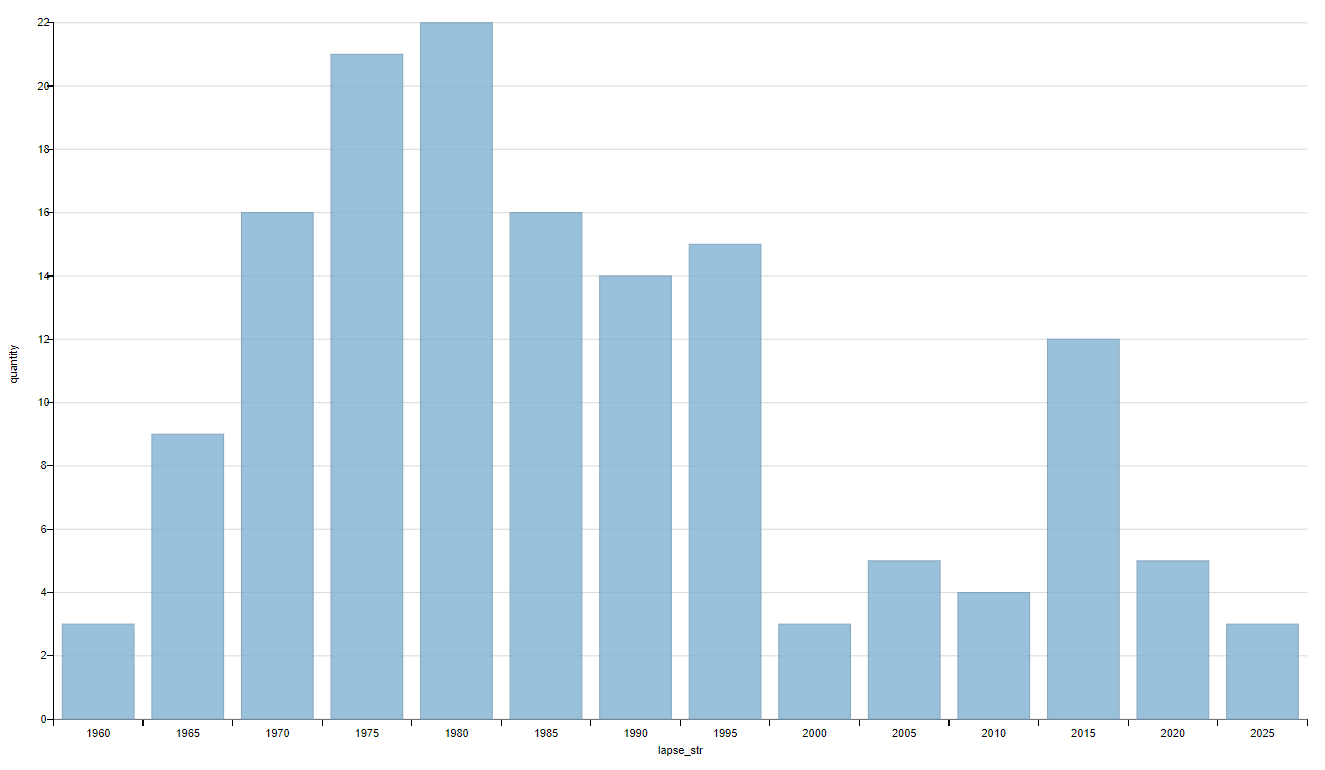
\includegraphics[width=\linewidth]{graphics/chapter/spacecraft_space_station/ImgRU.png}
  \caption[График Россия]{Визуализация количества запусков космических кораблей а России каждые 5 лет 2021 SPARQL}%
  \label{fig:launchesRussia5years}%
\end{figure*}

Горизонтальной ос\'{и} на рис.~\ref{fig:launchesRussia5years} отвечает переменая \mbox{\lstinline|?lapse_str|.} 
Если не преобразовывать число \lstinline|?lapse| 
в текстовую переменную \mbox{\lstinline|?lapse_str|}%
\sidenote[][]{
%
Преобразование числа в текст  
в третьей строке запроса~\ref{lst:launchesRussia5years}:\newline
\lstinline|(STR(?lapse) AS ?lapse_str)|.%
%
}, то ось~X имеет диапазон от 0 до 2200, 
вместо требуемого диапазона от 1960 до 2025 года, 
а результаты обозначаются точками с координатами (пятилетка, число запусков), 
и график становится нечитаемым. 

Из рис.~\ref{fig:launchesRussia5years} видно, 
что самый активный период развития отечественной космонавтики был в 1970--1995 годах.

Запрос~\ref{lst:launchesWorld} строит график~\ref{fig:launchesWorld} 
запусков космических кораблей в~мире по годам и странам.

\begin{lstlisting}[ language=SPARQL, 
                    numbers=none, 
                    caption={{\href{https://w.wiki/4bEu}{Запуски космических кораблей в мире}}\protect\footnotemark}, 
                    label=lst:launchesWorld 
                  ]
# Diagram of spacecraft launches by year and country
#defaultView:BarChart
SELECT ?year (COUNT(?obj) AS ?count) ?country ?countryLabel
WHERE {
  ?obj wdt:P17 ?country. # spacecraft belongs to country 
  ?obj wdt:P619 ?launch. # date of spacecraft launch
  BIND(str(YEAR(?launch)) AS ?year)
  
  SERVICE wikibase:label {bd:serviceParam wikibase:language "ru".}
}
GROUP BY ?year ?country ?countryLabel
\end{lstlisting}
%%%%%%%%%%%%%%%% Упражнение 2 %%%%%%%%%%%%%%%% 
\marginnote[-4cm]{%
В какое из десятилетий (1970-е, 1980-е, 1990-е или 2000-е) 
человечестро совершило наибольшее и наименьшее количество запусков космических кораблей?

См. ответ~\ref{answer:launches_world} на с.~\pageref{answer:launches_world}.
}
\footnotetext{Найдено \num{328} результатов в 2021 году. Ссылка на SPARQL-запрос: \href{https://w.wiki/4bEu}{https://w.wiki/4bEu}}

\begin{figure*}[h!]
  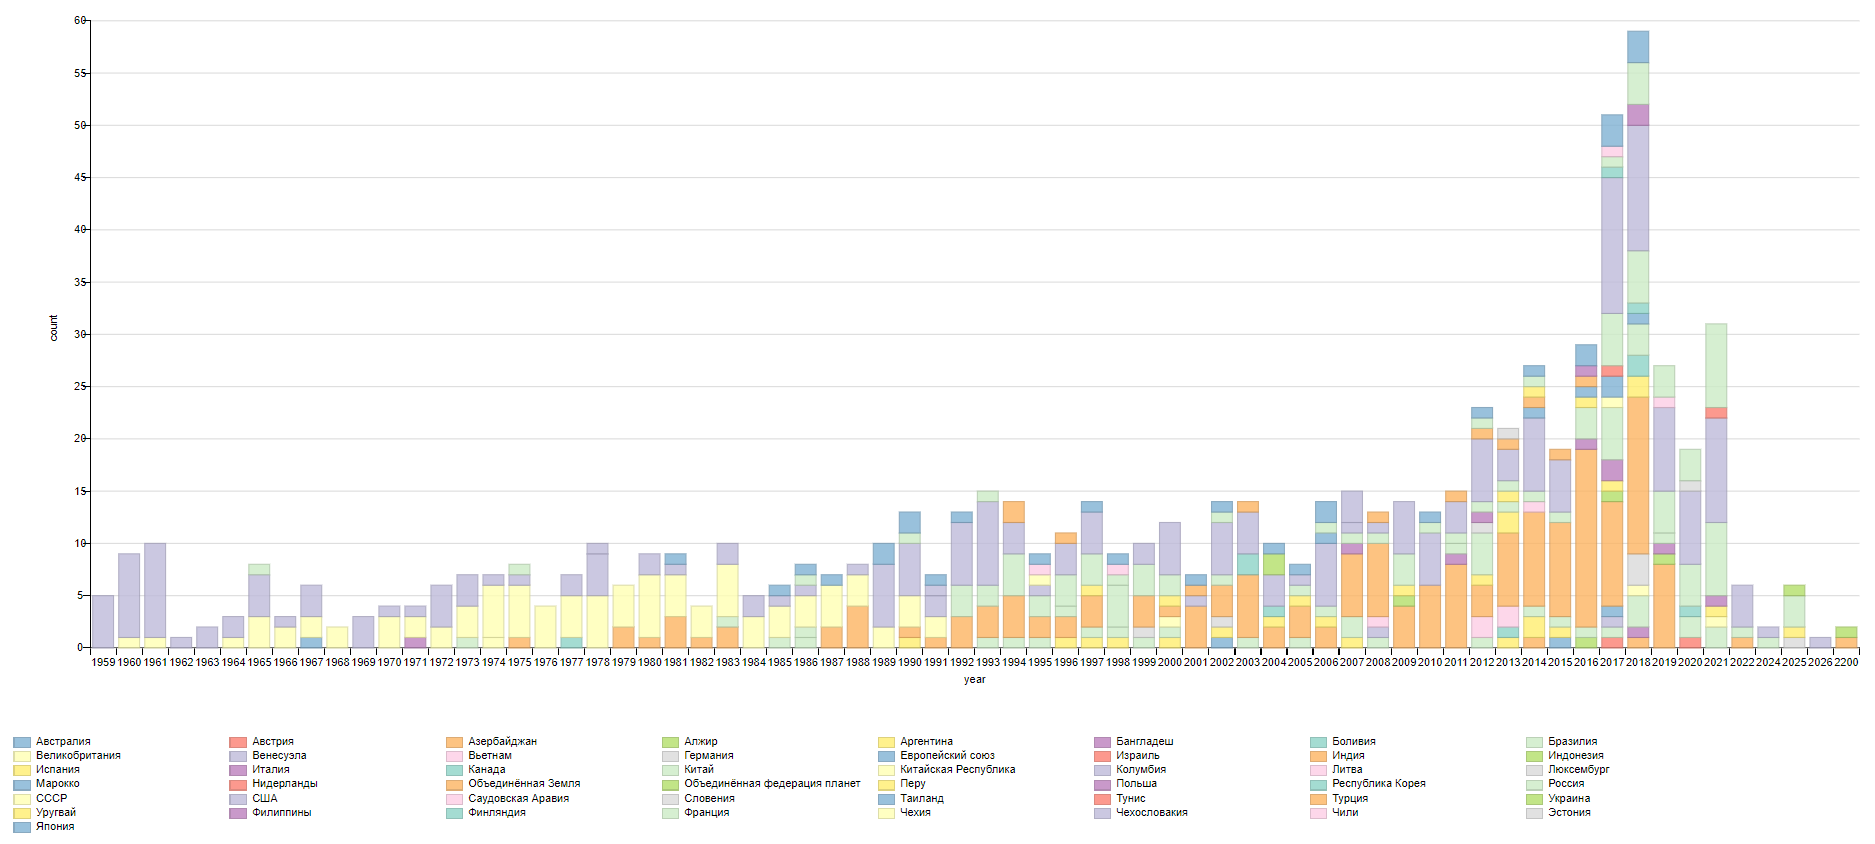
\includegraphics[width=\linewidth]{graphics/chapter/spacecraft_space_station/Visualization of the number of spacecraft launches by year and country 2021.png}
  \caption[График мир]{Визуализация количества запусков космических кораблей по годам и странам 2021 SPARQL}%
  \label{fig:launchesWorld}%
\end{figure*}
%
%%%%%%%%%%%%%%%% Упражнение 3 %%%%%%%%%%%%%%%% 
\marginnote[32pt]{Подсчитайте в Викиданных, в какой из стран~--- Россия, США, Индия или Китай~---  
было больше всего запусков космических кораблей с 2015 по 2020 год?
\newline
См. ответ~\ref{answer:launches_country} на с.~\pageref{answer:launches_country}.
}

Из рис.~\ref{fig:launchesWorld} видно, что больше всего космических аппаратов 
запускали Индия и США 
(только у них зафиксировано более 10 ежегодных запусков) в 2017--2018 годах. 
Пик запусков в мире был в 2018 году (59 запусков). 

По Викиданным российская космонавтика занимает средние позиции по количеству запусков, 
её численные показатели за 2016--2019 годы схожи с показателями СССР в 1970-е и 1980-е годы 
и составляют 3--5 запусков в год.

\section{Упражнения}
\begin{itemize}
  \item Постройте список кораблей, которые отправились или отправятся на \wdqName{Марс}{111}.
  \item Подсчитайте долю кораблей (нарисуйте график по десятилетиям), 
        отправленным на \wdqName{Марс}{111}, 
        по отношению к числу кораблей, отправленных на \wdqName{Луну}{405}.
  \item Подсчитайте количество \wdqName{успешных}{7632586} космических запусков 
      относительно \wdqName{неудачных}{1121708}.%
\marginnote[-32pt]{%
Например, у объекта \wdqName{<<космическая программа Луна>>}{192372} 
в свойстве \wdProperty{793}{<<ключевое событие>>} 
указано число успешных и неудачных запусков.%
}%
\end{itemize}
